\section{Modelli di regressione}
\subsection{Introduzione ai regressori}
I regressori sono dei modelli di machine learning il cui obiettivo è quello di prevedere un valore numerico continuo (in questo caso il valore delle emissioni).
I regressori vengono valutati sulla base di metriche quali, per esempio, l'errore quadratico medio (MSE), l'errore assoluto medio (MAE), e l'errore quadrato logaritmico medio (MSLE).

\subsection{Regressori utilizzati}
In questo lavoro sono stati utilizzati i seguenti regressori:
\begin{itemize}
    \item \textbf{Support Vector Regression (SVR)}\footnote{\href{https://scikit-learn.org/stable/modules/generated/sklearn.svm.SVR.html}{SVR}}{}
    \item \textbf{Decision Tree Regressor} \footnote{\href{https://scikit-learn.org/stable/modules/generated/sklearn.tree.DecisionTreeRegressor.html}{Decision Tree Regressor}}{}
    \item \textbf{Random Forest Regressor} \footnote{\href{https://scikit-learn.org/stable/modules/generated/sklearn.ensemble.RandomForestRegressor.html}{Random Forest Regressor}}{}
    \item \textbf{AdaBoost Regressor} \footnote{\href{https://scikit-learn.org/stable/modules/generated/sklearn.ensemble.AdaBoostRegressor.html}{AdaBoost Regressor}}{}
\end{itemize}
\subsubsection{Support Vector Regression (SVR)}
%add a footnote to SVM
La SVR è un algoritmo che estende il concetto di Support Vector Machine (SVM)\footnote{Algoritmi di classificazione che cercano di trovare un iperpiano ottimale per ottenere separabilità lineare}{} al caso della regressione.
\begin{figure}[H]
    \centering
    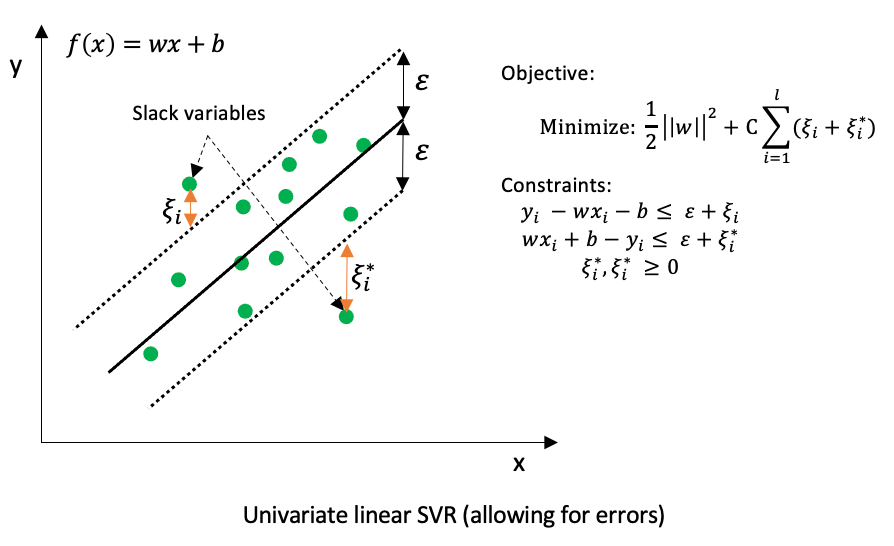
\includegraphics[scale=0.5]{images/SVR.png}
    \caption*{Esempio di SVR}
\end{figure} \newpage
\noindent In questo lavoro il modello è stato costruito usando gli iperparametri di default. Questi ultimi sono:
\begin{itemize}
    \item \textbf{kernel=rbf}: E' il tipo di Kernel\footnote{Funzione matematica usata per mappare i dati originali in uno spazio di dimensione superiore}{} utilizzato. Questo kernel valuta quanto due punti siano simili sulla base della loro distanza
    \item \textbf{degree=3}:  grado del polinomio utilizzato per la trasformazione dei dati nello spazio
    \item \textbf{gamma=scale}: coefficiente del kernel
    \item \textbf{coef0=0.0}: termine indipendente nel kernel
    \item \textbf{tol=0.001}: tolleranza per il criterio di arresto
    \item \textbf{C=1.0}: parametro di regolarizzazione
    \item \textbf{epsilon=0.1}:  controlla la tolleranza del modello nei confronti degli errori nella predizione
    \item \textbf{shrinking=True}: se abilitare o meno la riduzione del set di supporto
    \item \textbf{cache\_size=200}: dimensione della cache in MB
    \item \textbf{max\_iter=-1}: numero massimo di iterazioni. -1 indica nessun limite
\end{itemize}


\subsubsection{Decision Tree Regressor}

I Decision Tree Regressors sono modelli di regressione basati su alberi decisionali. Questi algoritmi suddividono ripetutamente il set di dati in base alle caratteristiche (features) per creare una struttura ad albero che rappresenta la relazione di decisione. Ogni nodo interno dell'albero rappresenta una decisione basata su una caratteristica, e le foglie dell'albero contengono i valori di output previsti.
\begin{figure}[H]
    \centering
    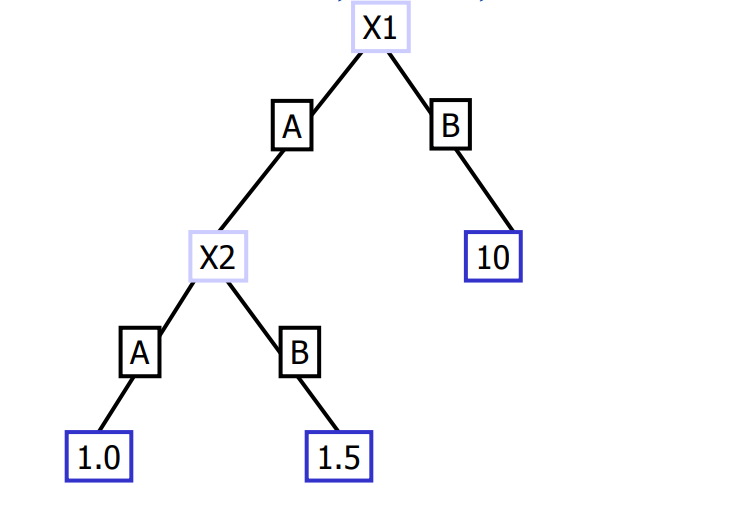
\includegraphics[scale=0.5]{images/DecisionTreeRegressor.png}
    \caption{Esempio di albero decisionale di regressione}
\end{figure}

\noindent In questo lavoro due iperparametri sono stati decisi all'atto della costruzione del modello:
\begin{itemize}
    \item \textbf{max\_depth=5}: profondità massima dell'albero
    \item \textbf{random\_state=3}:  controlla la casualità nell'addestramento del modello. Quando viene fissato a un numero intero specifico l'addestramento del modello sarà deterministico, cioè produrrà gli stessi risultati in ogni esecuzione
\end{itemize}
\noindent mentre gli altri iperparametri sono stati lasciati ai valori di default:
\begin{itemize}
    \item \textbf{criterion=squared\_error}: Criterio per stabilire la qualità di una suddivisione
    \item \textbf{splitter=best}: Strategia per scegliere la suddivisione in ogni nodo
    \item \textbf{min\_samples\_split=2}: Numero minimo di campioni richiesti per suddividere un nodo interno
    \item \textbf{min\_samples\_leaf=1}: Numero minimo di campioni richiesti per essere in una foglia
    \item \textbf{min\_weight\_fraction\_leaf=0.0}: La frazione minima dei campioni totali (pesati) necessaria affinché si verifichi un nodo foglia
    \item \textbf{max\_features=None}: Numero di features da considerare quando si cerca la migliore suddivisione. None indica tutte
    \item \textbf{max\_leaf\_nodes=None}: Numero massimo di foglie. None indica nessun limite
    \item \textbf{min\_impurity\_decrease=0.0}: Un nodo verrà suddiviso se questa suddivisione induce una diminuzione dell'impurità maggiore o uguale a questo valore
    \item \textbf{ccp\_alpha=0.0}: Parametro di complessità usato per la potatura
    \item \textbf{monotonic\_constraints=None}: Vincoli monotoni sui valori delle features
\end{itemize}

\subsubsection{Random Forest Regressor}
I Random Forest Regressors sono modelli di regressione basati su alberi decisionali. Vengono costruiti su più alberi decisionali che combinano le loro previsioni per ottenere una previsione più accurata e stabile.
\begin{figure}[H]
    \centering
    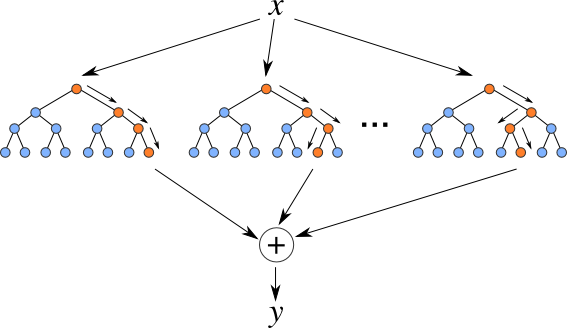
\includegraphics[scale=0.5]{images/RandomForestRegressor.png}
    \caption{Esempio di Random Forest Regresor}
\end{figure}

\noindent In questo lavoro tre iperparametri sono stati decisi all'atto della costruzione del modello:
\begin{itemize}
    \item \textbf{n\_estimators=500}: numero di alberi nella foresta
    \item \textbf{max\_depth=5}: profondità massima dell'albero
    \item \textbf{random\_state=3}:  controlla la casualità nell'addestramento del modello. Quando viene fissato a un numero intero specifico l'addestramento del modello sarà deterministico, cioè produrrà gli stessi risultati in ogni esecuzione
\end{itemize}

\noindent mentre gli altri iperparametri sono stati lasciati ai valori di default:
\begin{itemize}
    \item \textbf{criterion=squared\_error}: Criterio per stabilire la qualità di una suddivisione
    \item \textbf{min\_samples\_split=2}: Numero minimo di campioni richiesti per suddividere un nodo interno
    \item \textbf{min\_samples\_leaf=1}: Numero minimo di campioni richiesti per essere in una foglia
    \item \textbf{min\_weight\_fraction\_leaf=0.0}: La frazione minima dei campioni totali (pesati) necessaria affinché si verifichi un nodo foglia
    \item \textbf{max\_features=1}: Numero di features da considerare quando si cerca la migliore suddivisione
    \item \textbf{max\_leaf\_nodes=None}: Numero massimo di foglie. None indica nessun limite
    \item \textbf{min\_impurity\_decrease=0.0}: Un nodo verrà suddiviso se questa suddivisione induce una diminuzione dell'impurità maggiore o uguale a questo valore
    \item \textbf{ccp\_alpha=0.0}: Parametro di complessità usato per la potatura
    \item \textbf{bootstrap=True}: Se utilizzare il bootstrap per la costruzione degli alberi
    \item \textbf{oob\_score=False}: Se calcolare l'errore out-of-bag
    \item \textbf{n\_jobs=None}: Numero di lavori da eseguire in parallelo. None indica 1
    \item \textbf{warm\_start=False}: Se utilizzare la soluzione precedente come inizializzazione
    \item \textbf{max\_samples=None}: Numero massimo di campioni da utilizzare per la costruzione di ciascun albero. None indica tutti
    \item \textbf{monotonic\_constraints=None}: Vincoli monotoni sui valori delle features
\end{itemize}
\newpage
\subsubsection{AdaBoost Regressor}
L'AdaBoost Regressor è un modello basato sull'algoritmo di boosting AdaBoost\footnote{Crea un modello forte combinando modelli più deboli, ognuno allenato su diverse parti del dataset}{}. Questo algoritmo costruisce un modello di previsione combinando più modelli di previsione più deboli.
\begin{figure}[H]
    \centering
    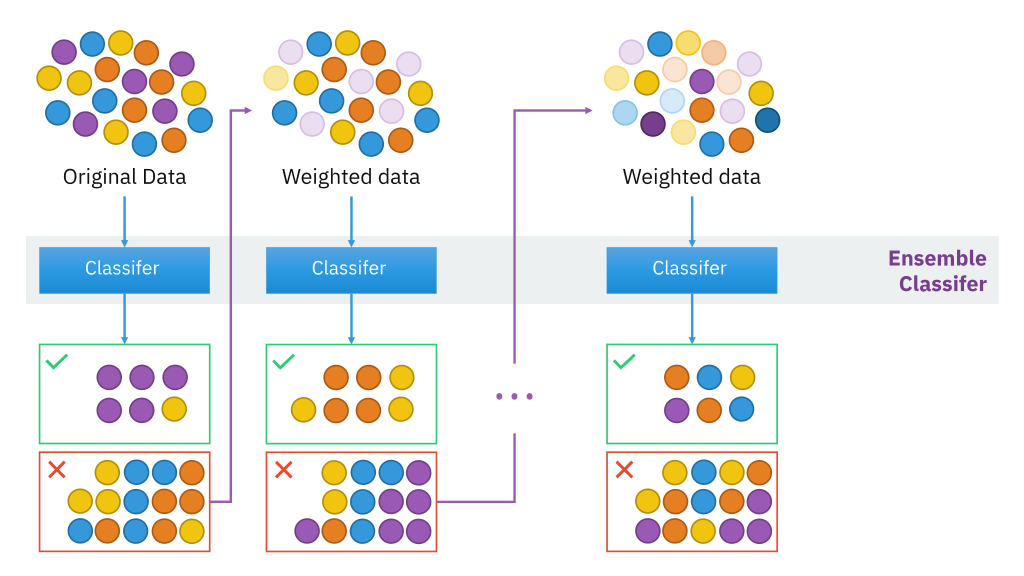
\includegraphics[scale=0.4]{images/AdaBoost.png}
    \caption{Struttura di modello basato su AdaBoost}
\end{figure}

\noindent In questo lavoro due iperparametri sono stati decisi all'atto della costruzione del modello:

\begin{itemize}
    \item \textbf{n\_estimators=500}: numero di stimatori
    \item \textbf{random\_state=3}:  controlla la casualità nell'addestramento del modello. Quando viene fissato a un numero intero specifico l'addestramento del modello sarà deterministico, cioè produrrà gli stessi risultati in ogni esecuzione
\end{itemize}

\noindent mentre gli altri iperparametri sono stati lasciati ai valori di default:
\begin{itemize}
    \item \textbf{estimator=None}: stimatore base. Se None, viene utilizzato DecisionTreeRegressor
    \item \textbf{learning\_rate=1.0}: tasso di apprendimento
    \item \textbf{loss=linear}: funzione di perdita
\end{itemize}

